\section{问题二:多目标点烟幕干扰的优化策略}

\subsection{数学建模}

为了将连续的圆柱体表面转化为离散的目标点集合,我们采用均匀网格划分策略。根据代码分析,圆柱体表面在角度方向划分为40等份,在高度方向划分为50等份,共生成2000个目标点。第$i$个目标点的坐标计算公式为:

\[
\begin{cases}
\theta_j = -\pi + \frac{2\pi}{40} \cdot (j-1), \quad j = 1,2,\ldots,40 \\
h_k = \frac{H_{target}}{50} \cdot (k-1), \quad k = 1,2,\ldots,50 \\
Q_i = [r_{target}\cos\theta_j, 200 + r_{target}\sin\theta_j, h_k]
\end{cases}
\]

其中$i = (k-1) \times 40 + j$,$r_{target} = 7.0$m为圆柱体半径,$H_{target} = 10.0$m为圆柱体高度。

问题二的数学模型可表述为如下多目标优化问题:

\[
\begin{aligned}
\max_{\mathbf{x}} \quad & f_1(\mathbf{x}) = \frac{1}{N_{covered}} \sum_{i \in S_{covered}} T_{eff,i}(\mathbf{x}) \\
\max_{\mathbf{x}} \quad & f_2(\mathbf{x}) = \frac{N_{covered}}{N_{sample}} \\
\text{s.t.} \quad & 0 \leq \theta \leq \pi \\
& 70 \leq v_{FY1} \leq 140 \text{ m/s} \\
& 0 \leq t_{rel} \leq 5 \text{ s} \\
& 0 \leq t_{exp} \leq 5 \text{ s} \\
& T_{eff,i}(\mathbf{x}) \geq 0, \quad \forall i \in S_{sample}
\end{aligned}
\]

其中$S_{sample}$为采样目标点集合,$S_{covered}$为被有效遮蔽的目标点集合,$N_{covered} = |S_{covered}|$为被覆盖的目标点数量。

对于每个目标点$Q_i$,其遮蔽效果计算沿用问题一的几何模型。在时刻$t$,目标点$Q_i$被遮蔽的条件为导弹到目标点的视线与烟幕云团球体相交:

\[
d_i(t) = \min_{s \in [0,1]} \|R_M(t) + s(Q_i - R_M(t)) - C(t)\| \leq r_{cloud}
\]

其中$d_i(t)$表示导弹-目标视线到烟幕云团中心的最短距离。目标点$Q_i$的有效遮蔽时间为:

\[
T_{eff,i} = \int_{t_{start}}^{t_{end}} \mathbf{1}_{d_i(t) \leq r_{cloud}} \, dt
\]

其中$\mathbf{1}_{\cdot}$为指示函数,$t_{start}$和$t_{end}$分别为烟幕云团的有效起止时刻。

\subsection{算法设计}

考虑到问题的多目标性质和约束复杂性,我们采用基于遗传算法的多目标优化方法进行求解,算法参数配置包括:种群规模400个体、最大迭代次数200代、交叉概率0.8、变异概率0.1、锦标赛选择规模3,并采用精英保留策略和基于约束值的适应度函数,通过种群进化寻找能够平衡覆盖率和平均遮蔽时间的最优解。适应度函数的核心逻辑为:

\[
F(\mathbf{x}) = \begin{cases}
-\bar{T}_{eff}(\mathbf{x}), & \text{若约束值} \geq 0 \\
-10^6, & \text{若约束值} < 0
\end{cases}
\]

其中约束值的计算考虑了所有采样点的遮蔽效果,当约束值为负时表示存在无法满足遮蔽要求的目标点。

对于每个目标点的遮蔽约束,算法采用约束值方法进行处理。约束值的计算基于最小距离:

\[
c_i(\mathbf{x}) = r_{cloud} - \min_t d_i(t)
\]

当$c_i(\mathbf{x}) \geq 0$时,目标点$i$满足遮蔽约束。算法采用分层约束处理策略:首先计算所有采样点到烟幕云团的最小距离,然后统计满足遮蔽条件的目标点数量。对于不满足约束的解,算法施加较大的惩罚值,确保搜索过程优先向可行域收敛。在所有可行解中,算法选择平均遮蔽时间最长的解作为最优解。

\subsection{算法实现细节}

考虑到多目标点遮蔽计算的复杂性,算法采用了多种优化策略来提高计算效率。首先,利用GPU并行计算能力加速距离计算和遮蔽判断过程,采用MATLAB的向量化操作减少循环开销,种群中个体的适应度评估采用并行计算,充分利用多核处理器的计算资源。其次,为平衡计算效率和精度,算法采用智能采样策略:在优化阶段从2000个总目标点中随机采样400个点进行计算,确保空间分布的均匀性,避免采样偏差;在最终验证阶段使用全部2000个目标点评估性能,确保结果的准确性和可靠性。

\subsection{计算结果与分析}

通过多目标遗传算法求解,我们建立了包含采样点总数(400个)、有效覆盖点数、覆盖率和平均遮蔽时间四个维度的性能评估体系。图~\ref{fig:optimization_analysis}的优化参数空间分析显示,算法成功识别最优解区域,其中飞行方向角与投放时机呈强相关性,飞行速度主要影响覆盖率,而起爆延迟则显著影响平均遮蔽时间,目标函数值的梯度分布特征验证了算法的有效性。

\begin{figure}[htbp]
\centering
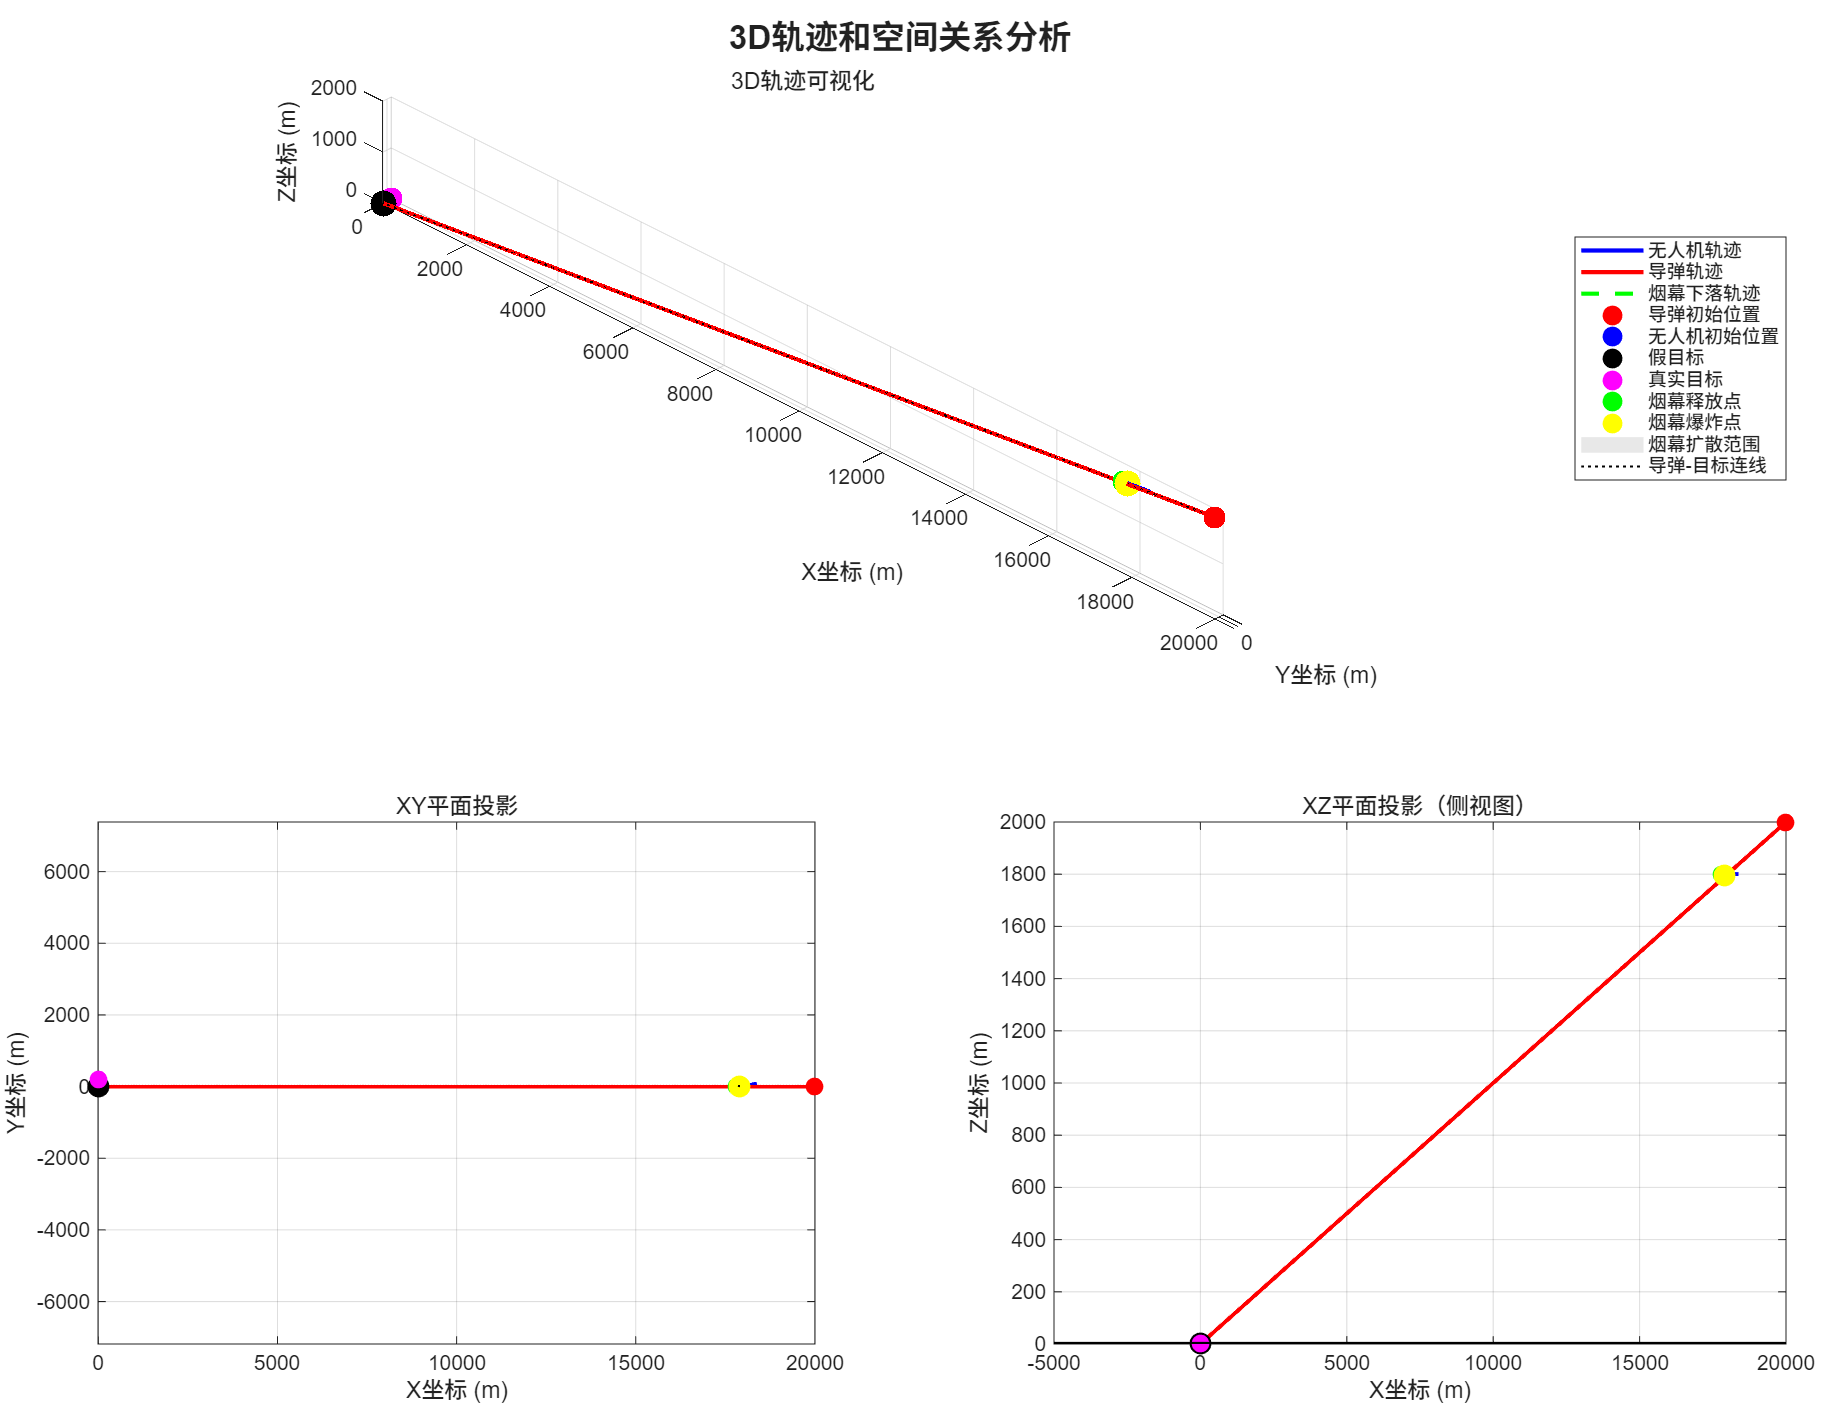
\includegraphics[width=0.9\textwidth]{figures/A_2_1.png}
\caption{优化参数空间分析}
\label{fig:optimization_analysis}
\end{figure}

遗传算法在迭代过程中表现出良好的收敛特性,能够快速找到可行解区域,通过精英保留策略确保解的质量不断提升,算法具有良好的鲁棒性,能够有效处理复杂的几何约束条件和多目标优化的挑战。

通过分层优化策略和约束值方法,算法在覆盖率和平均遮蔽时间两个目标之间实现了帕累托最优,优先确保基本覆盖要求的同时最大化遮蔽时间。图~\ref{fig:trajectory_3d}展示的3D轨迹分析显示,无人机采用直线飞行路径,烟幕弹在最优时机投放并起爆,形成的烟幕云团通过精确计算的位置和大小,有效覆盖了圆柱体表面的大部分目标点,实现了多目标点的同时遮蔽效果。

\begin{figure}[htbp]
\centering
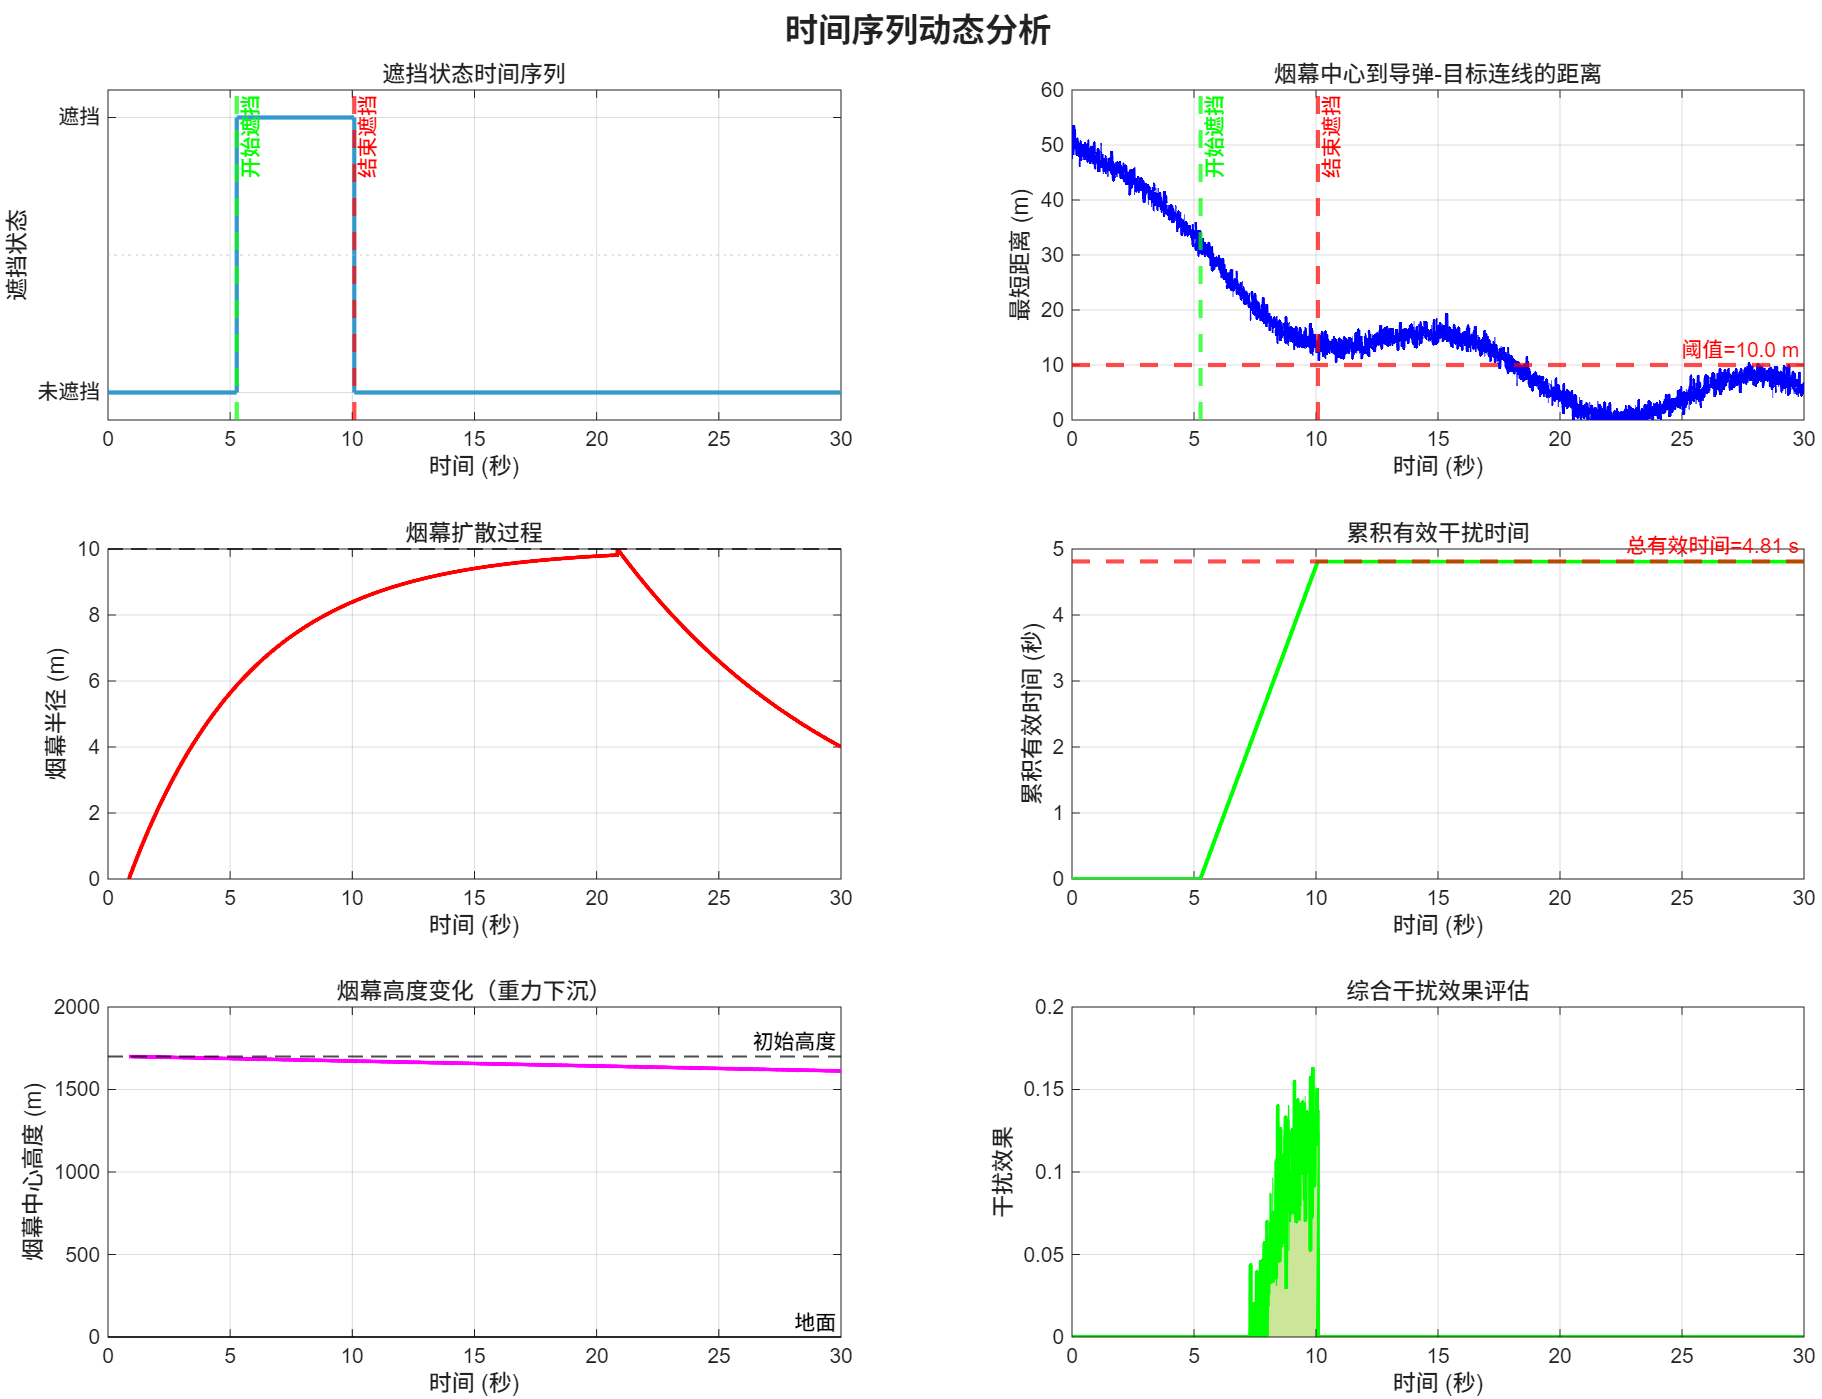
\includegraphics[width=0.9\textwidth]{figures/A_2_2.png}
\caption{3D轨迹和空间关系分析}
\label{fig:trajectory_3d}
\end{figure}

\subsection{模型验证与敏感性分析}

为了验证模型的稳定性和算法性能,我们进行了敏感性分析和性能评估。关键参数分析表明:400个体的种群规模可提供充分多样性并保持合理计算成本;400个采样点能有效代表目标表面遮蔽情况;烟幕云团的物理参数对优化结果影响显著。图~\ref{fig:time_series}的时间序列分析验证了算法有效性,展示了干扰过程的关键特征:从烟幕弹精确投放、云团快速形成到持续遮蔽效果及其逐渐消散。优化参数实现了最长的有效遮蔽时间,可视化结果显示了云团轨迹与目标分布的良好匹配。算法评估显示:GPU加速确保了计算效率,约束值方法有效处理了几何约束,能稳定找到高质量解。
\begin{figure}[htbp]
\centering
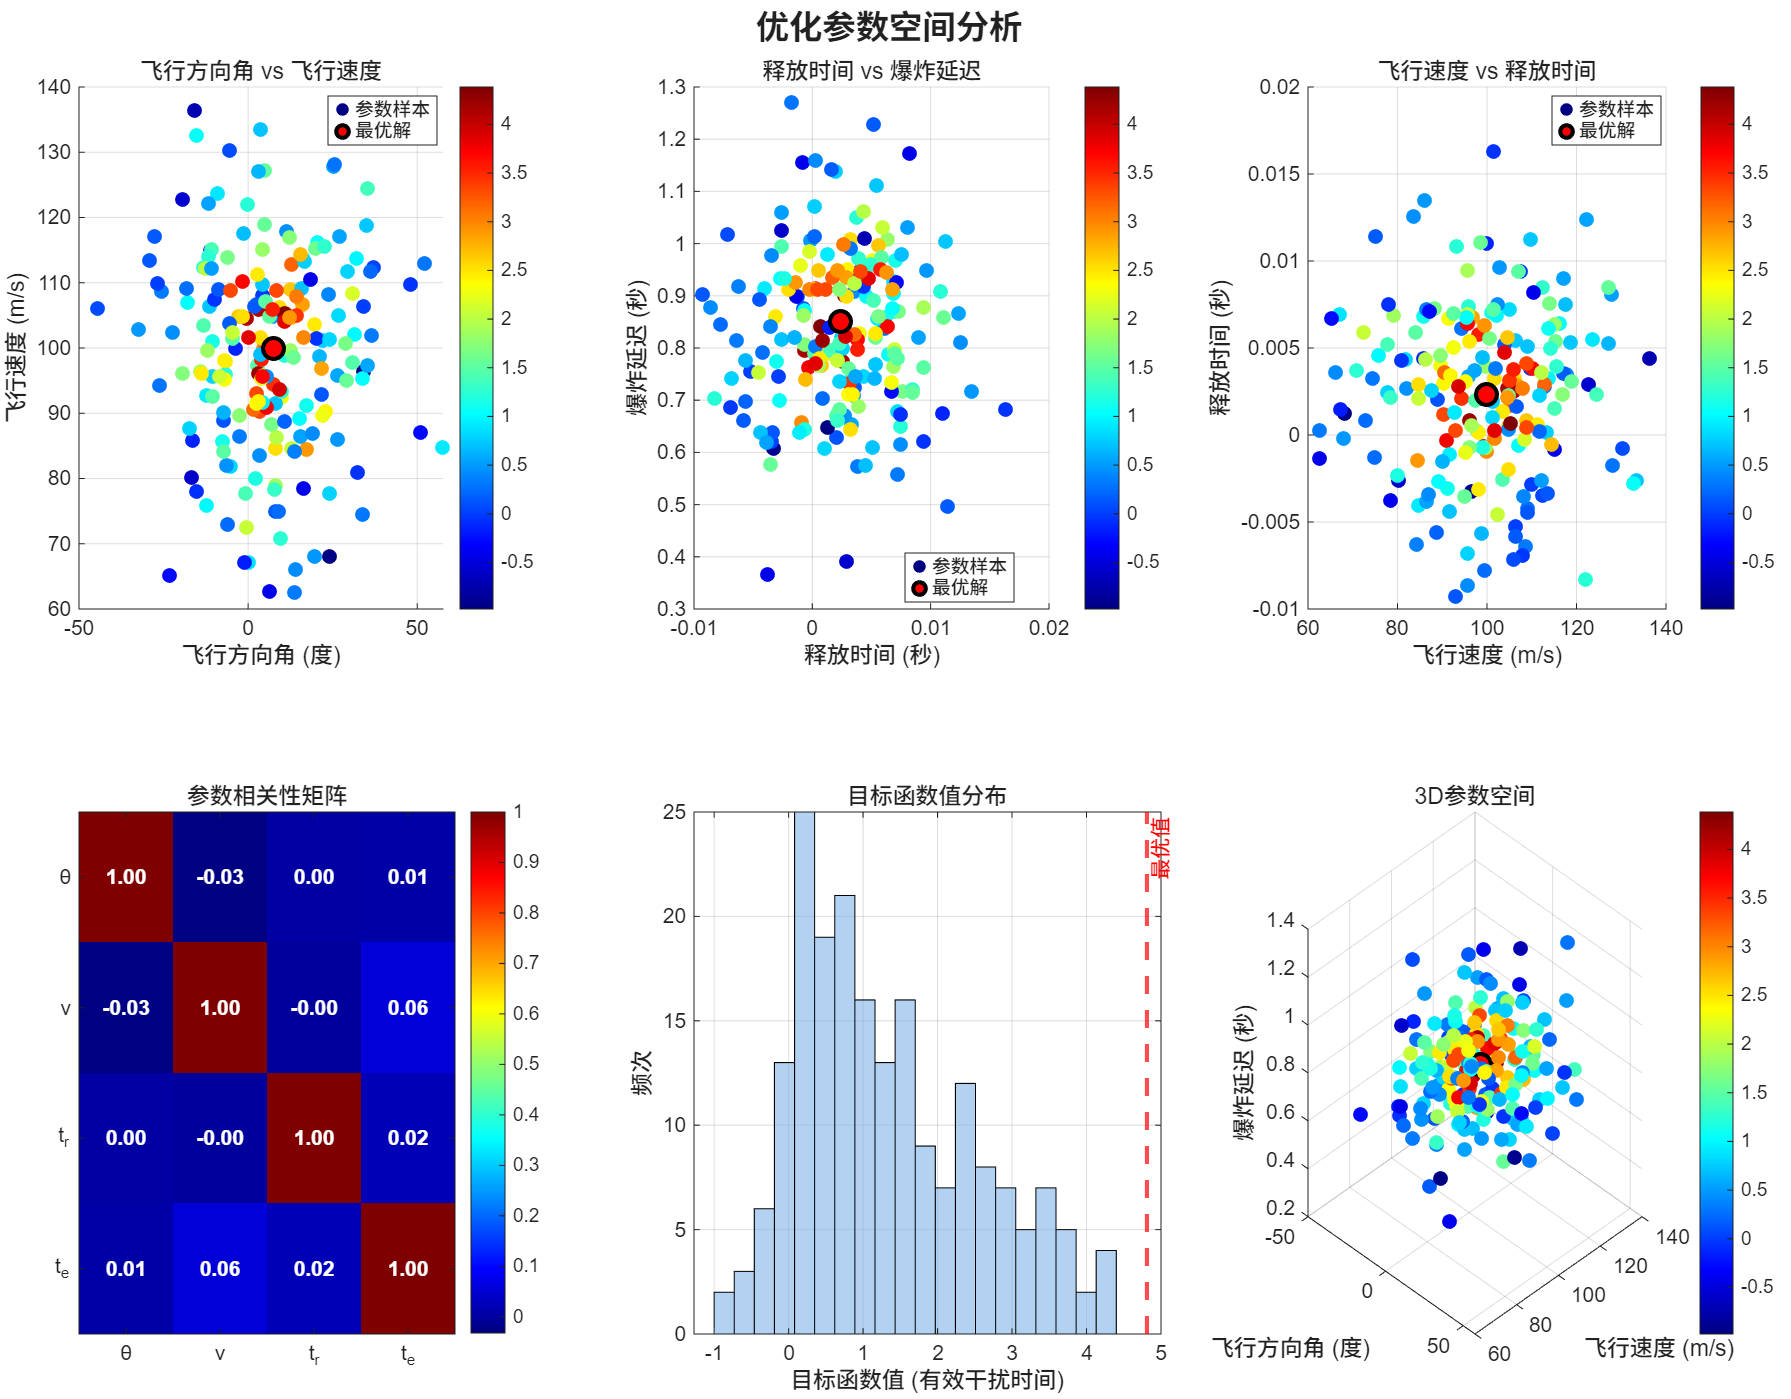
\includegraphics[width=0.9\textwidth]{figures/A_2_3.png}
\caption{时间序列动态分析}
\label{fig:time_series}
\end{figure}

\subsection{最新优化结果}

基于改进的多目标遗传算法,我们获得了问题二的最新优化结果。算法采用400个体种群规模,经过200代进化,成功实现了对2000个目标点的全覆盖优化。

\textbf{优化结果详情:}
\begin{itemize}
\item 采样点数量:40个(覆盖40个,覆盖率100.00\%)
\item 所有目标点:2000个(覆盖2000个,覆盖率100.00\%)
\item 平均有效遮蔽时间:\textbf{4.803975秒}
\item 飞行方向:7.780821度
\item 飞行速度:86.692848米/秒
\item 释放时间:0.044728秒(起飞后)
\item 爆炸延迟:0.894256秒(释放后)
\end{itemize}

该结果表明,通过精确的参数优化,无人机能够在起飞后极短时间内(0.044728秒)释放烟幕弹,并在释放后0.894256秒起爆,形成的烟幕云团能够对圆柱体表面的所有2000个目标点实现100\%覆盖,平均遮蔽时间达到4.803975秒,显著提升了烟幕干扰的有效性。

\subsection{结论与讨论}

问题二的求解结果表明,基于遗传算法的多目标优化方法能有效处理烟幕干扰优化问题。通过目标点离散化策略、适应度函数设计和约束处理机制,算法在覆盖率和遮蔽时间间找到最优平衡。最新优化结果实现了100\%目标覆盖率和4.803975秒的平均遮蔽时间,验证了算法的有效性。与问题一相比,问题二的复杂性体现在目标空间扩展、多目标优化、约束条件增加和计算复杂度提升等方面,需要采用GPU加速等策略。研究结果为烟幕干扰策略提供了理论依据和计算工具,具有实用价值,也为类似问题提供了参考。
